% ------------------------------------------------------------------ %
% Examination of a Bayesian approach to inverse kinematics.
% Andrew J. Pohl, Matthew R. Schofield & Reed Ferber
% Submitted to Journal of Biomechanics March 2021
% SupplementaryMaterialA.tex
% ------------------------------------------------------------------ %
\documentclass{article}
\usepackage{setspace}
% ------------------------------------------------------------------ %
% Examination of a Bayesian approach to inverse kinematics.
% Andrew J. Pohl, Matthew R. Schofield & Reed Ferber
% Submitted to Journal of Biomechanics March 2021
% SupplementaryMaterial Structure
% structure.tex
% ------------------------------------------------------------------ %
%% Package inclusion
\usepackage[running]{lineno} % Line Numbers


 \usepackage[authoryear]{natbib}
\bibliographystyle{model5-names}

% SI 
\usepackage{siunitx}
% Hyper refferences
\usepackage{hyperref}

% Packages for tables
\usepackage{multirow}

% Packages for figures
\usepackage{subcaption}	

% Math Packages
\usepackage{amsmath,amsfonts,stmaryrd,amssymb, bm} 
\DeclareMathOperator*{\argmin}{argmin} 

\usepackage{enumerate} % Custom item numbers for enumerations

\usepackage[ruled]{algorithm2e} % Algorithms

\usepackage[framemethod=tikz]{mdframed} % Allows defining custom boxed/framed environments

\usepackage{listings} % File listings, with syntax highlighting
\lstset{
	basicstyle=\ttfamily, % Typeset listings in monospace font
}

%----------------------------------------------------------------
%	DOCUMENT MARGINS
%----------------------------------------------------------------

\usepackage{geometry} % Required for adjusting page dimensions and margins

\geometry{
	paper=letterpaper, % Paper size, change to letterpaper for US letter size
	top=2.5cm, % Top margin
	bottom=3cm, % Bottom margin
	left=2.5cm, % Left margin
	right=2.5cm, % Right margin
	headheight=14pt, % Header height
	footskip=1.5cm, % Space from the bottom margin to the baseline of the footer
	headsep=1.2cm, % Space from the top margin to the baseline of the header
	%showframe, % Uncomment to show how the type block is set on the page
}

%-------------------------------------------------------------------------
%	FONTS
%-------------------------------------------------------------------------

\usepackage[utf8]{inputenc} % Required for inputting international characters
\usepackage[T1]{fontenc} % Output font encoding for international characters

\usepackage{XCharter} % Use the XCharter fonts

%---------------------------------------------------------------------------
%	EMPHASISE ENVIRONMENT
%---------------------------------------------------------------------------

% Usage:
% \begin{emphasise}
%	\begin{verbatim}
%		$ ls
%		
%		Applications	Desktop	...
%	\end{verbatim}
% \end{commandline}

\mdfdefinestyle{emphasise}{
	leftmargin=10pt,
	rightmargin=10pt,
	innerleftmargin=15pt,
	middlelinecolor=black!50!white,
	middlelinewidth=2pt,
	frametitlerule=false,
	backgroundcolor=black!5!white,
	frametitle={Command Line},
	frametitlefont={\normalfont\sffamily\color{white}\hspace{-1em}},
	frametitlebackgroundcolor=black!50!white,
	nobreak,
}

% Define a custom environment for command-line snapshots
\newenvironment{emphasise}{
	\medskip
	\begin{mdframed}[style=emphasise]
}{
	\end{mdframed}
	\medskip
}

%--------------------------------------------------------------------------
%	FILE CONTENTS ENVIRONMENT
%--------------------------------------------------------------------------

% Usage:
% \begin{file}[optional filename, defaults to "File"]
%	File contents, for example, with a listings environment
% \end{file}

\mdfdefinestyle{file}{
	innertopmargin=1.6\baselineskip,
	innerbottommargin=0.8\baselineskip,
	topline=false, bottomline=false,
	leftline=false, rightline=false,
	leftmargin=2cm,
	rightmargin=2cm,
	singleextra={%
		\draw[fill=black!10!white](P)++(0,-1.2em)rectangle(P-|O);
		\node[anchor=north west]
		at(P-|O){\ttfamily\mdfilename};
		%
		\def\l{3em}
		\draw(O-|P)++(-\l,0)--++(\l,\l)--(P)--(P-|O)--(O)--cycle;
		\draw(O-|P)++(-\l,0)--++(0,\l)--++(\l,0);
	},
	nobreak,
}

% Define a custom environment for file contents
\newenvironment{file}[1][File]{ % Set the default filename to "File"
	\medskip
	\newcommand{\mdfilename}{#1}
	\begin{mdframed}[style=file]
}{
	\end{mdframed}
	\medskip
}

%--------------------------------------------------------------------------
%	NUMBERED QUESTIONS ENVIRONMENT
%--------------------------------------------------------------------------

% Usage:
% \begin{question}[optional title]
%	Question contents
% \end{question}

\mdfdefinestyle{question}{
	innertopmargin=1.2\baselineskip,
	innerbottommargin=0.8\baselineskip,
	roundcorner=5pt,
	nobreak,
	singleextra={%
		\draw(P-|O)node[xshift=1em,anchor=west,fill=white,draw,rounded corners=5pt]{%
		Question \theQuestion\questionTitle};
	},
}

\newcounter{Question} % Stores the current question number that gets iterated with each new question

% Define a custom environment for numbered questions
\newenvironment{question}[1][\unskip]{
	\bigskip
	\stepcounter{Question}
	\newcommand{\questionTitle}{~#1}
	\begin{mdframed}[style=question]
}{
	\end{mdframed}
	\medskip
}

%-------------------------------------------------------------------------
%	WARNING TEXT ENVIRONMENT
%-------------------------------------------------------------------------

% Usage:
% \begin{warn}[optional title, defaults to "Warning:"]
%	Contents
% \end{warn}

\mdfdefinestyle{warning}{
	topline=false, bottomline=false,
	leftline=false, rightline=false,
	nobreak,
	singleextra={%
		\draw(P-|O)++(-0.5em,0)node(tmp1){};
		\draw(P-|O)++(0.5em,0)node(tmp2){};
		\fill[black,rotate around={45:(P-|O)}](tmp1)rectangle(tmp2);
		\node at(P-|O){\color{white}\scriptsize\bf !};
		\draw[very thick](P-|O)++(0,-1em)--(O);%--(O-|P);
	}
}

% Define a custom environment for warning text
\newenvironment{warn}[1][Warning:]{ % Set the default warning to "Warning:"
	\medskip
	\begin{mdframed}[style=warning]
		\noindent{\textbf{#1}}
}{
	\end{mdframed}
}

%------------------------------------------------------------------------
%	INFORMATION ENVIRONMENT
%------------------------------------------------------------------------

% Usage:
% \begin{info}[optional title, defaults to "Info:"]
% 	contents
% 	\end{info}

\mdfdefinestyle{info}{%
	topline=false, bottomline=false,
	leftline=false, rightline=false,
	nobreak,
	singleextra={%
		\fill[black](P-|O)circle[radius=0.4em];
		\node at(P-|O){\color{white}\scriptsize\bf i};
		\draw[very thick](P-|O)++(0,-0.8em)--(O);%--(O-|P);
	}
}

% Define a custom environment for information
\newenvironment{info}[1][Info:]{ % Set the default title to "Info:"
	\medskip
	\begin{mdframed}[style=info]
		\noindent{\textbf{#1}}
}{
	\end{mdframed}
}
 

% Label figures/tables starting with A
\renewcommand{\thefigure}{A\arabic{figure}}
\setcounter{figure}{0}

\renewcommand{\thetable}{A\arabic{table}}
\setcounter{table}{0}

\title{Supplementary Material A - Additional Results} 

\author{Andrew J. Pohl, Matthew R. Schofield \&  Reed Ferber} 

\date{University of Calgary \today} 
%--------------------------------------------------------------------- %

\begin{document}
\linenumbers
\maketitle 

\doublespacing

The following appendix contains additional results cited within the body of the accompanying article.  All research code can be found at: \href{https://github.com/AndyPohlNZ/BayesKin}{https://github.com/AndyPohlNZ/BayesKin}.
\section{Model Performance}
Performance of each model on identifying the underling pose parameters when the the least-squares solution of each simulation are used as initial values for MCMC sampling (Bayesian Models) are presented for 1 and 2 link chains in Figures \ref{fig:StripChart_SingleLink_True} and \ref{fig:StripChart_DoubleLink_True} respectfully. Results for the 3-link problem are found within the body of the main text. Clearly all models are unbiased yet the Bayesian model with the 2nd set of priors (equation (5) in the main text) demonstrates considerably less variance than the other models.

\begin{figure}
\centering
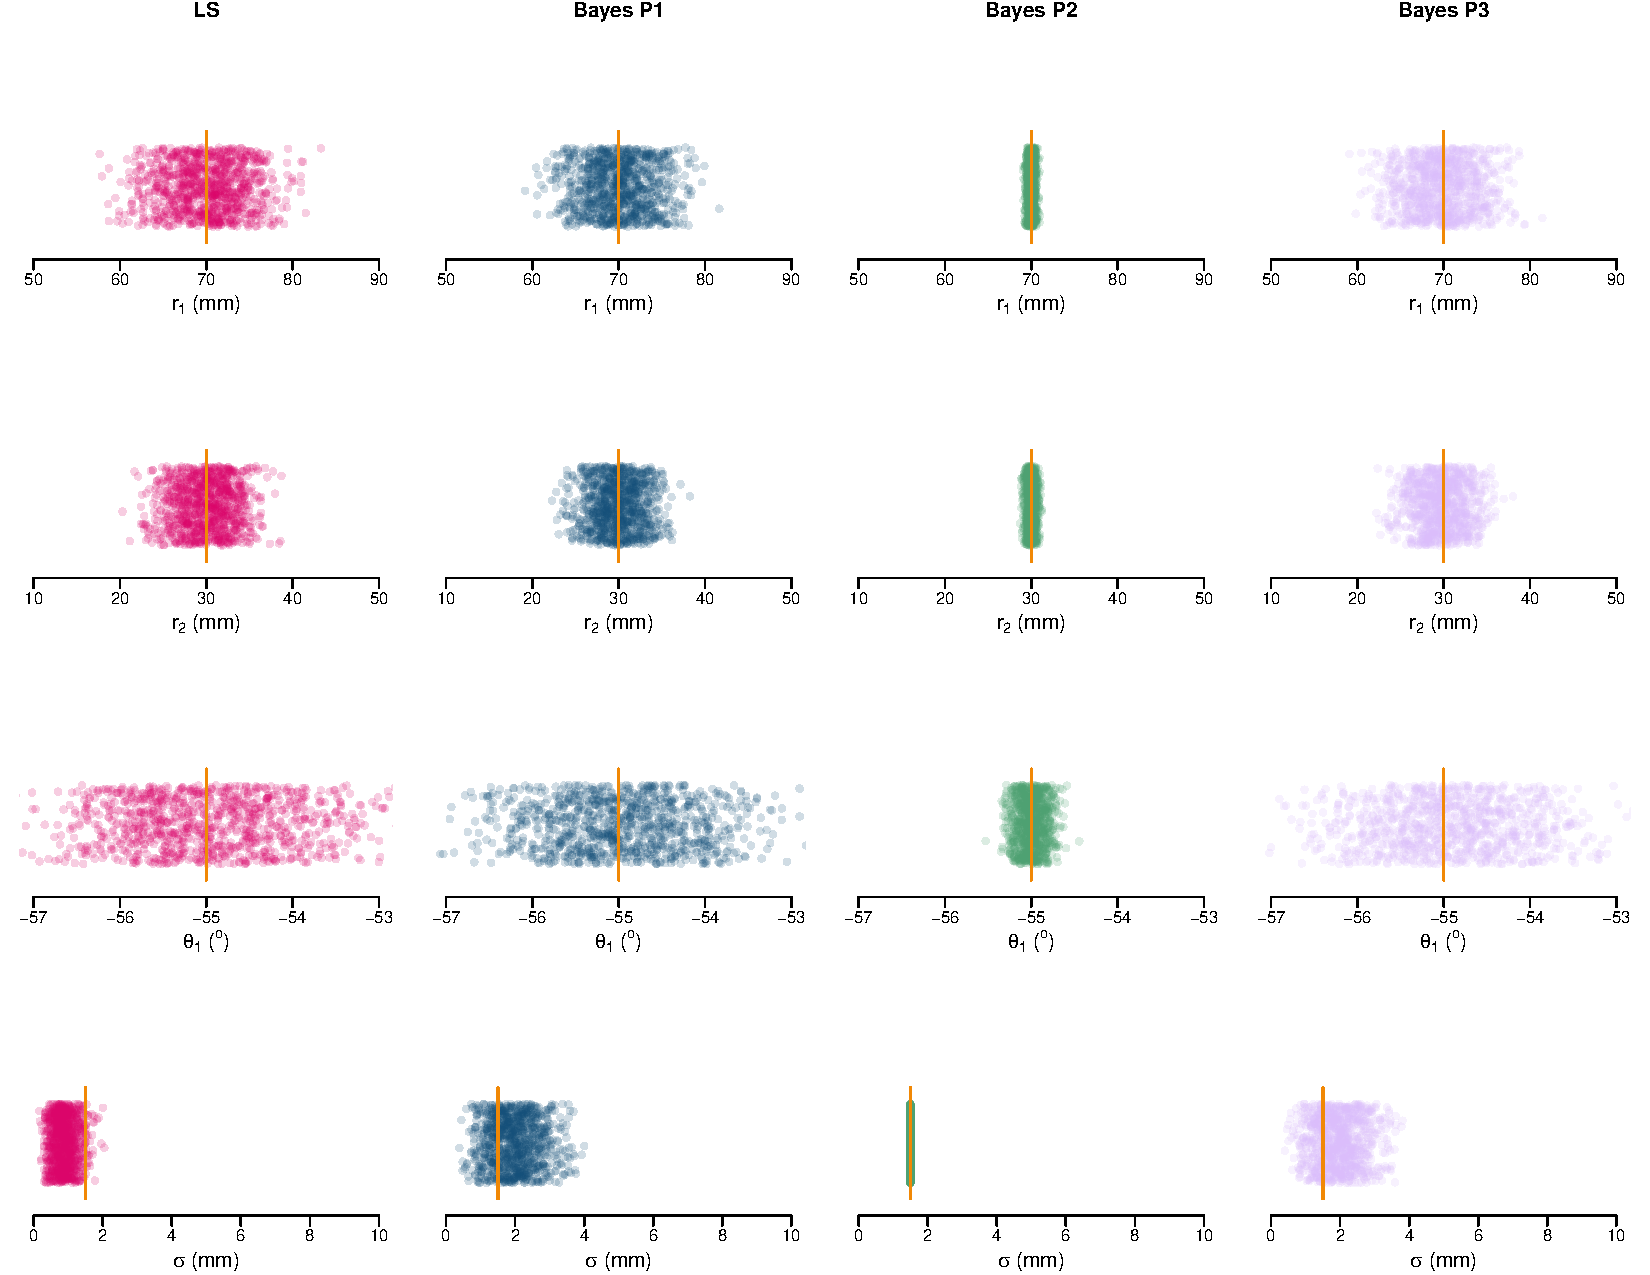
\includegraphics[width=\textwidth]{./Figures/SingleLink_StripChart.pdf}
\caption{Performance of the estimators from each model (columns) on each parameter (rows) for 1000 single link simulations where initial values were specified using the true values.  True values for each parameter identified in orange.}
\label{fig:StripChart_SingleLink_True}
\end{figure}

\begin{figure}
\centering
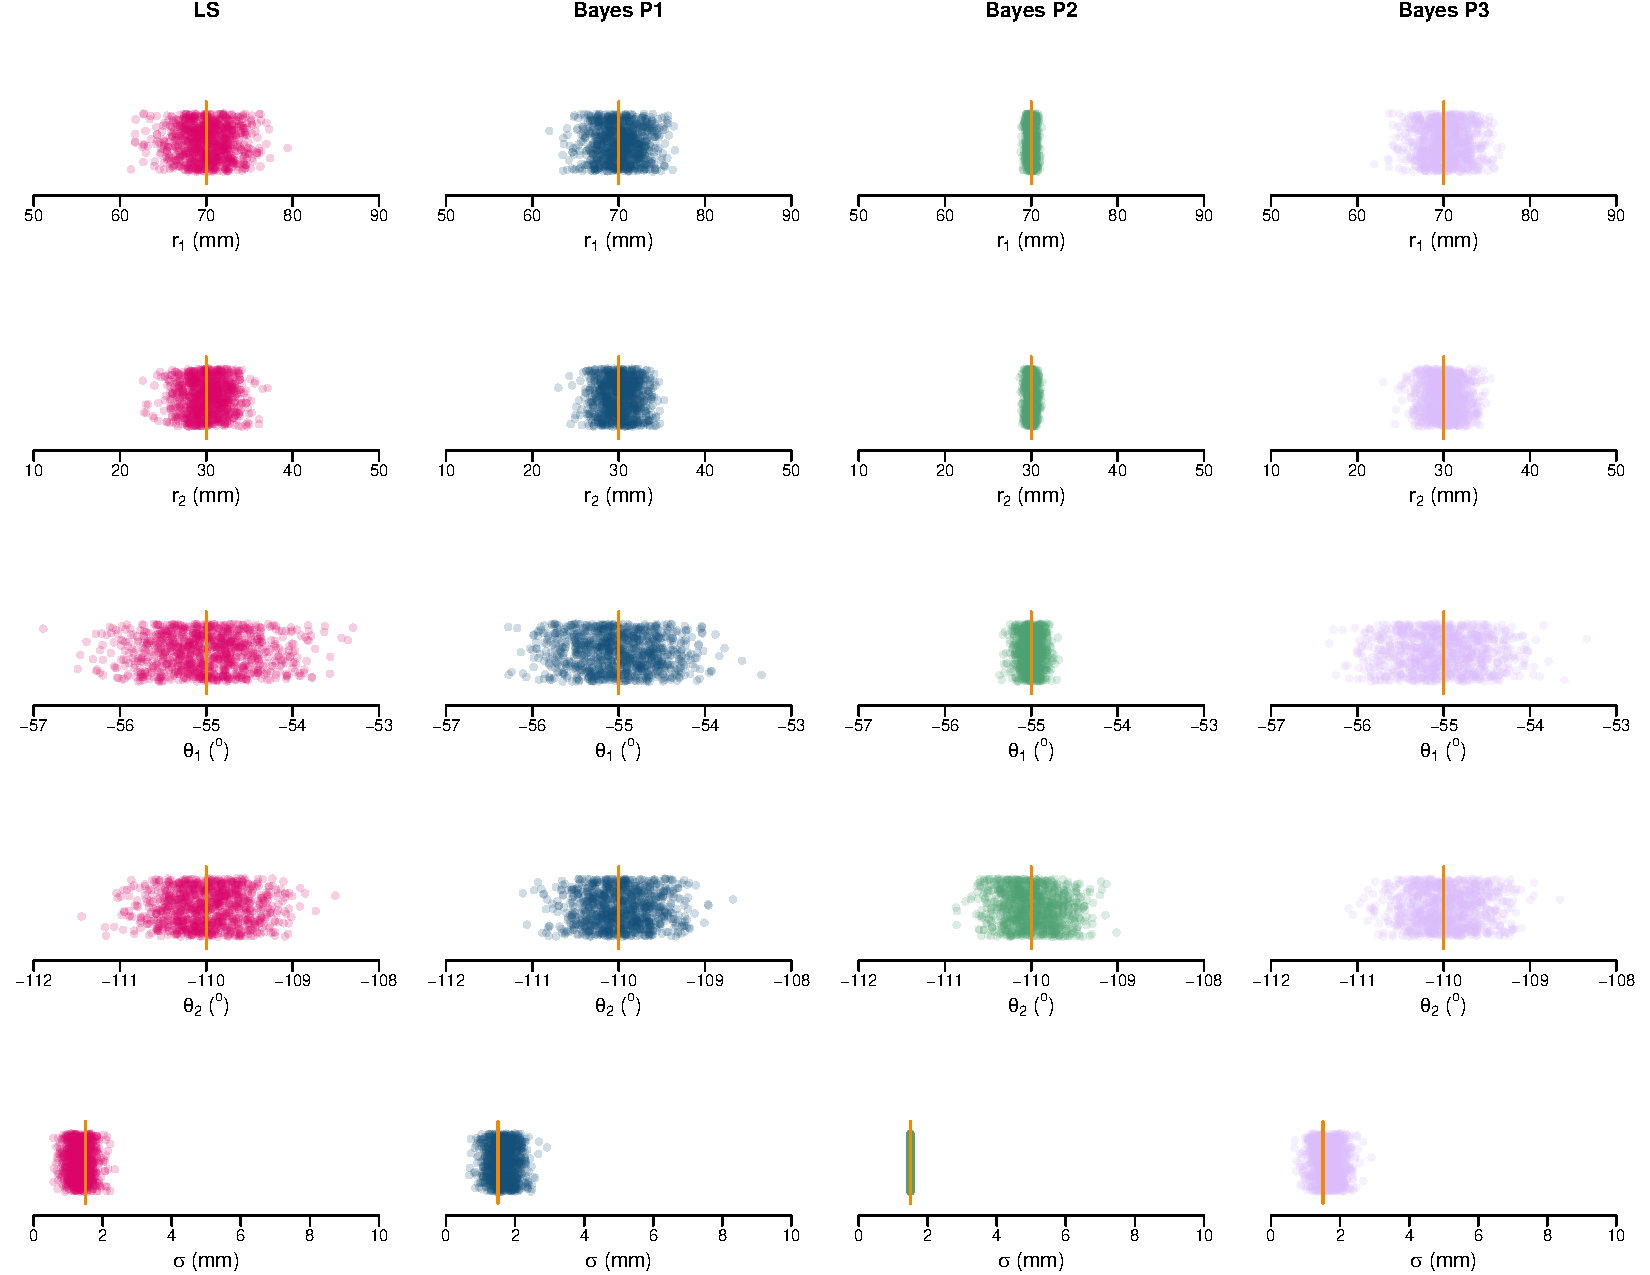
\includegraphics[width=\textwidth]{./Figures/DoubleLink_StripChart.pdf}
\caption{Performance of the estimators from each model (columns) on each parameter (rows) for 1000 double link simulations where initial values were specified using the true values.  True values for each parameter identified in orange.}
\label{fig:StripChart_DoubleLink_True}
\end{figure}

\section{Computational Time}
The average computational time for each model is presented in Table \ref{tab:Comptime_Truevals}  In general it took an order of magnitude longer to obtain 10000 MCMC samples from the Bayesian posterior than to solve the non linear optimization problem to obtain the LS estimator.  Both numerical optimisation and MCMC sampling were performed on the same mobile workstation (P51, Intel i7-7820HQ 2.6GHz processor, 32GB RAM; Lenovo, Hong Kong.).
\begin{table}
   \centering
   %\resizebox{}{!}
   \caption{Average (SD) computation time (\si{\second}) for each model on 1, 2 and 3 link chains.}
   \label{tab:Comptime_Truevals}
\end{table}

\section{Markov Chain Monte Carlo}
In general sound convergence and efficient sampling were obtained for each of the Bayesian models for 1, 2 and 3 link problems.  This is highlighted in the fact that $< 0.1$\% of simulations were excluded on the basis of poor convergence with a $\hat{R}$ statistic greater than 1.1 units \citep{brooks_general_1998}.  Exemplary trace plots are provided for a 3 link problem in Figure \ref{fig:traceplot}. Table \ref{tab:ESS_table} outlines the mean effective sample size for each parameter along with the mean $\hat{R}$ statistic.  The fact that we have large numbers of effective samples and a $\hat{R}$ close to 1 gives us confidence in the parameter values obtained, the exception being estimates for the measurement noise parameter ($\sigma$) obtained using the 2nd set of priors.  This due to the extremely informative nature of the prior distribution for this model.

\begin{figure}
\centering
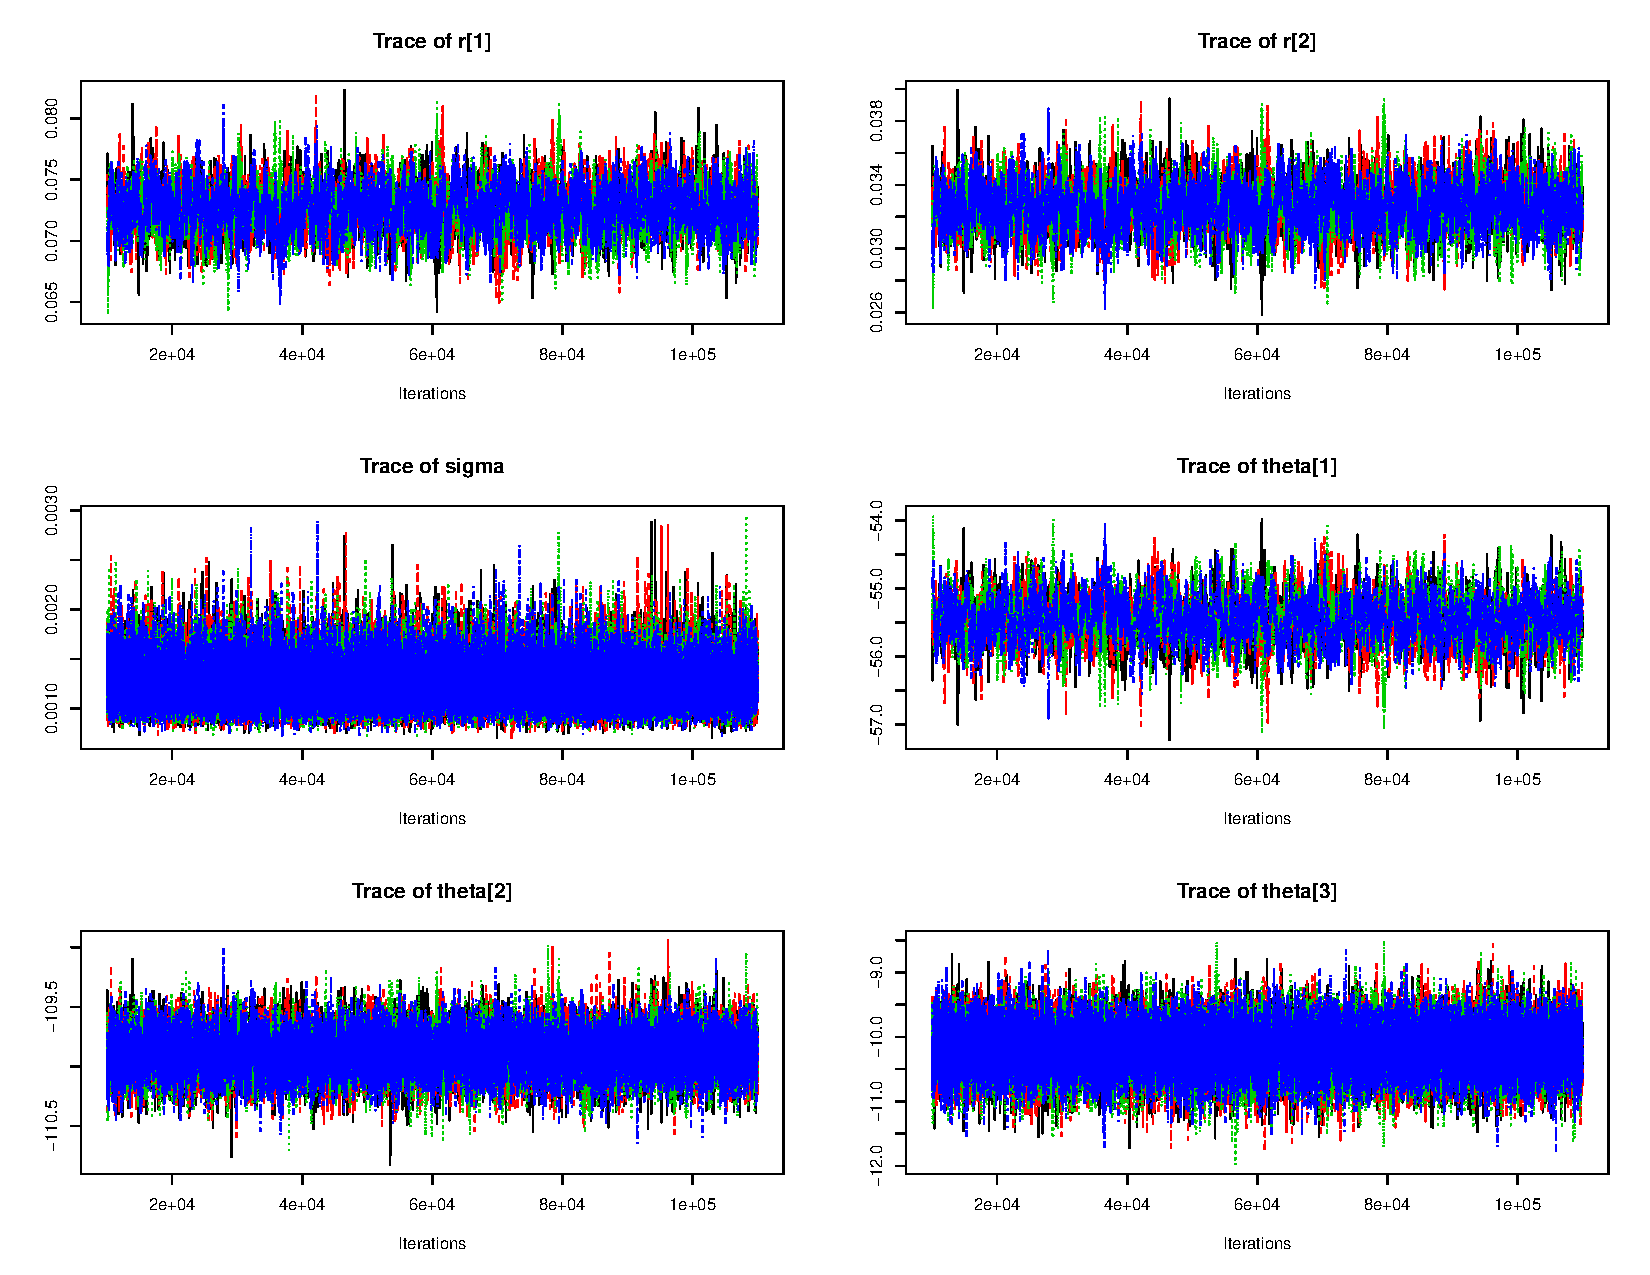
\includegraphics[width=\textwidth]{./Figures/traceplot.pdf}
\caption{Typical traceplot showing MCMC sampling for each parameter in the 3-link problem.  Each of four independent MCMC chains is depicted in a differing color.}
\label{fig:traceplot}
\end{figure}


\begin{table}
   \centering
   \resizebox{\textwidth}{!}{%
   \begin{tabular}{l l c c cc c cc c}
       \hline
       \multicolumn{2}{c}{Pose} & \multicolumn{2}{c}{Bayes P1} &&\multicolumn{2}{c}{Bayes P2}&&\multicolumn{2}{c}{Bayes P3} \\
      						&& ESS &$\hat{R}$ && ESS & $\hat{R}$ && ESS & $\hat{R}$ \\
  		\hline
  		\multirow{4}{*}{1-Link} & $r_1$ & 3105.3 (217.3) & 1.004 (0.005) && 60821.5 (890.7)& 1.000 (0.001) && 3121.6 (201.0)& 1.004 (0.005) \\
  									& $r_2$ & 3212.5 (248.1) & 1.004 (0.006) && 66222.6 (990.2) & 1.000 (0.001) && 3238.5 (225.2) & 1.004 (0.004) \\
  									& $\theta_1$ & 3045.4 (212.6) & 1.004 (0.005) && 55826.2 (734.6) & 1.000 (0.001) && 3065.7 (195.8) & 1.004 (0.004)\\
  									& $\sigma$ & 11205.9 (2175.0) & 1.003 (0.006) && 0.0 (0.0) & 1.000 (0.001) && 11394.9 (1926.2) & 1.003 (0.005) \\
       \hline
       \multirow{5}{*}{2-Link} & $r_1$ & 4229.9 (124.1) & 1.002 (0.001) && 45433.2 (738.6) & 1.000 (0.001) && 3310.4 (115.3) & 1.002 (0.001) \\
  									& $r_2$ & 4281.1 (126.1) &  1.001 (0.001) && 42263.9 (680.0) & 0.000 (0.001) && 3270.4 (106.4) & 1.002 (0.001)\\
  									& $\theta_1$ & 3995.9 (108.1) & 1.002 (0.001) && 34862.1 (501.9) & 1.000 (0.001) && 3046.1 (92.9) & 1.002 (0.001) \\
  									& $\theta_2$ & 18101.3 (1023.3) & 1.000 (0.001) && 63292.2 (1111.3) & 1.000 (0.001) && 12891.0 (812.5) & 1.000 (0.001)\\
  									& $\sigma$ & 34083.8 (2252.0) & 1.000 (0.001) && 0.0 (0.0) & 1.000 (0.001) && 30393.7 (2321.5) & 1.000 (0.001) \\
  	  \hline
       \multirow{6}{*}{3-Link} & $r_1$ & 2961.1 (93.3) & 1.002 (0.001) && 32534.5 (639.1) & 1.000 (0.001) && 1732.4 (67.9) & 1.004 (0.001)\\
  									& $r_2$ & 3003.34 (95.9) & 0.002 (0.001) && 30606.2 (576.9) & 1.000 (0.001) && 1693.7 (63.1) & 1.004 (0.002) \\
  									& $\theta_1$ & 2792.9 (79.0) & 1.002 (0.001) && 23195.1 (396.2) & 1.000 (0.001) && 1552.6 (50.6) & 1.004 (0.003) \\
  									& $\theta_2$ & 11821.0 (670.9) & 1.000 (0.001) && 47623.6 (961.1) & 1.000 (0.001) && 6136.4 (416.9) & 1.001 (0.001)\\
  									& $\theta_3$ & 20366.4 (1045.1) & 1.000 (0.001) && 62508.2 (1206.1) & 1.000 (0.001) && 12175.2 (820.3) & 1.001 (0.001) \\
  									& $\sigma$ & 40926.7 (2426.6) & 1.000 (.001) && 0.0 (0.0) & 1.000 (0.001) && 32230.4 (2722.3) & 1.000 (0.001) \\
  	\hline  	  

   \end{tabular}
   }
   \caption{Average (SD) effective sample size (ESS) and R hat statistic $\hat{R}$ for each of the Bayesian models.}
   \label{tab:ESS_table}
\end{table}

\bibliography{References.bib}

\end{document}
